
\documentclass[11pt,landscape]{report}
\usepackage{graphicx}
\usepackage{amssymb}
\usepackage[colorlinks]{hyperref}
\usepackage{tocloft}


\newcommand{\SupNum}{2}
\textwidth = 10 in
\textheight = 7.0 in
\oddsidemargin = -0.5 in
\evensidemargin = -0.5 in
\topmargin = -0.5 in
\headheight = 0.0 in
\headsep = 0.0 in
\footskip = 0.65 in
\parskip = 0.2in
\parindent = 0.0in


\makeatletter
\renewcommand{\thefigure}{\ifnum \c@chapter>\z@ \thechapter.\fi S\SupNum{}--\@arabic\c@figure}
\renewcommand*\l@figure{\@dottedtocline{1}{1.5em}{3.3em}}
\renewcommand{\thesection}{}
\renewcommand\section{\@startsection {section}{1}{-5.6mm}%
                                   {-3.5ex \@plus -1ex \@minus -.2ex}%
                                   {2.3ex \@plus.2ex}%
                                   {\normalfont\Large\bfseries}}

\makeatother


\newcommand{\ArticleName}{``An Assessment of Sibship Reconstruction \\
Programs with Simulated Microsatellite Data''}

\author{Eric C. Anderson\thanks{\em Fisheries Ecology Division, Southwest Fisheries Science Center, National Marine Fisheries Service, NOAA, Santa Cruz, CA} \and 
Anthony Almudevar\thanks{{\em Department of Biostatistics and Computational Biology,University of Rochester Medical School, Rochester, NY}}
}



\newcommand{\nosibs}{{NoSibs}}
\newcommand{\allhalf}{{AllHalf}}
\newcommand{\allpathalf}{{AllPatHalf}}
\newcommand{\sfsnoh}{{SmallSGs}}
\newcommand{\sfswh}{{SmallSGs\_H}}
\newcommand{\slfsgnoh}{{BigSGs}}
\newcommand{\slfsgwh}{{BigSGs\_H}}
\newcommand{\onelargenoh}{{OneBig}}
\newcommand{\onelargewh}{{OneBig\_H}}
\newcommand{\lottalarge}{{LottaLarge}}

\newcommand{\PD}{\mathrm{PD}}
\newcommand{\PDT}{\mathrm{PD^T}}
\newcommand{\PDS}{\mathrm{PD_S}}
\newcommand{\PDST}{\mathrm{PD_S^T}}
\newcommand{\W}{\mathrm{PD_{AP}}} % W for wrong! = PD from assignment problem on a set cover
\newcommand{\WT}{\mathrm{PD_{AP}^T}}
\newcommand{\FIG}{Figure}

\newcommand{\colony}{{\sc colony}}
\newcommand{\prt}{{\sc prt}}
\newcommand{\kinalyzer}{{\sc kinalyzer}}
\newcommand{\familyfinder}{{\sc familyfinder}}



% get TOC spacing onto one page
\setlength\cftparskip{2pt}
\setlength\cftbeforepartskip{2pt}



\title{Supplement \SupNum{} to Article:\\
\ArticleName\\
\mbox{}\\
{\em Partition Distance Scatterplots} }




\begin{document}
\maketitle
\section{Overview/Orientation}
This supplement contains all the partition distance scatterplots for all the pairwise comparisons between different sibship inference methods, broken down over different scenarios, genotyping error rates, and partition distances. Here is an example, with a legend plot next to it.
\begin{center}
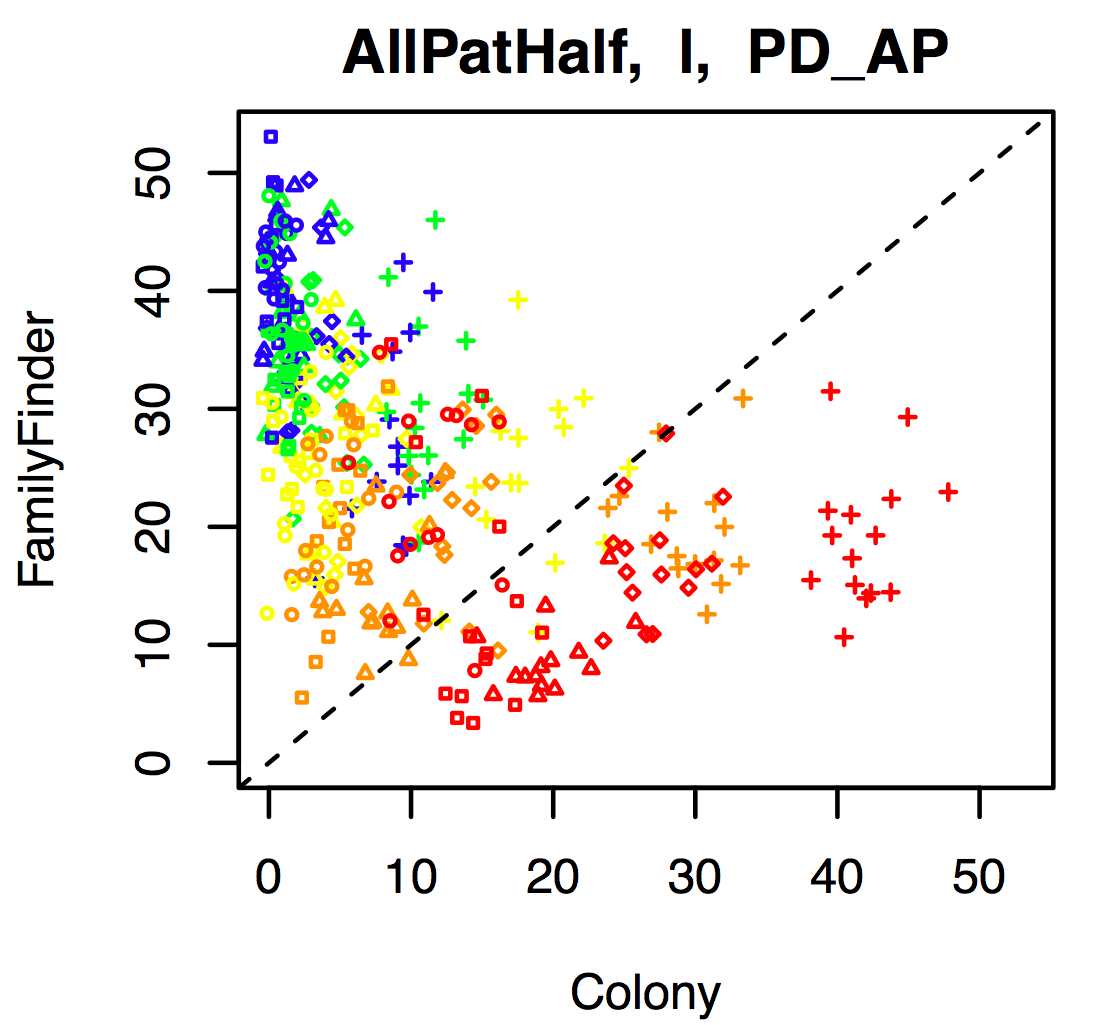
\includegraphics[width=.3\textwidth]{smearo_example.png}
~~~~~~~~~~~~~~~~~~~~~~~
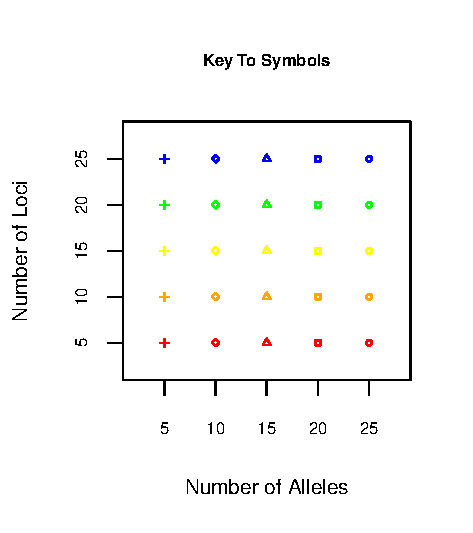
\includegraphics[width=.27\textwidth]{smearo_key.pdf}
\end{center}
The title of each plot has a comma separated string.  The first value is the true sibship configuration, and it denotes one of 
\nosibs,
\allhalf,
\allpathalf,
\sfsnoh,
\sfswh,
\slfsgnoh,
\slfsgwh,
\onelargenoh,
\onelargewh, or
\lottalarge.
The second value is ``n'', ``l'', or ``h,'' according to whether the data were simulated with no genotyping errors, a low genotyping error rate ($d=0.02,~m=0.01$), or a high genotyping error rate ($d=0.07,~m=0.03$), respectively.
The third value denotes the type of the partition distance used: PD\_AP = $\W$, PD\_S = $\PDS$, PD\_AP\^{}T = $\WT$, PD\_S\^{}T = $\PDST$.

The colors and shapes of plotting symbols represent the number of loci and alleles respectively.  Cooler colors correspond to more loci and hotter colors to few loci.  Rounder shapes correspond to more alleles and ``pointier'' shapes correspond to fewer alleles.  Here is a mnemonic: with fewer loci and fewer alleles you are more likely to get burned or pricked when you try to estimate sibling structure.  The coloring and the plot characters try to reflect this.  

Save a tree. Please don't print this out.  View it on your computer.
\newpage  
\tableofcontents

\newpage
\listoffigures

\input{../../tmp/plots/smearograms/latex_commands_for_smearograms.tex}

\end{document}